% ===================================================================
% UVic Physics & Astronomy Thesis Template
% -------------------------------------------------------------------
% This is the only .tex file you need to edit at the top level.
%   1. Choose your class options below.
%   2. Fill in your thesis details (title, name, committee, ...).
%   3. Edit the files in frontmatter/ (abstract, acknowledgements,
%      dedication).
%   4. Replace the example chapters in content/ with your own.
%
% The compiled example PDF (thesis.pdf) explains every feature used
% here. See uvicphysastro.cls for full option documentation.
% ===================================================================

\documentclass[
  degree=masters,           % masters | phd
  bibliography=natbib,      % none | natbib | biblatex
  % bibstyle=authoryear,    % biblatex style (bibliography=biblatex only)
  % spacing=double,         % onehalf (default) | double
  % floatfraction=0.5,      % lower (e.g. 0.01) = more float-only pages
  % draft=true,             % line numbers, label keys, todo notes, timestamp
  % listoftables=false,     % only if your thesis contains no tables
  % listoffigures=false,    % only if your thesis contains no figures
  % headings=centered,      % left (default) | centered: preliminary-page headings
]{uvicphysastro}

% -------------------------------------------------------------------
% Thesis details
% -------------------------------------------------------------------
\thesistitle{An Example Thesis Made With \LaTeX\ for Astronomy Students}
\thesisauthor{A Hopeful Graduate}   % your legal name, exactly as UVic has it
\thesisyear{2026}                   % year of completion
% Previously awarded credentials (optional; delete to show none)
\thesisdegrees{%
  B.Sc., University of WhoKnowsWhere, 2053\\
  M.Sc., University of AnotherOne, 2054%
}
% Supervisory committee: \panelist{Name}{Role}{Department}
% Do not list your external examiner or the exam chair.
\thesiscommittee{%
  \panelist{Dr. R.\ Supervisor Main}{Supervisor}{Department of Physics and Astronomy}%
  \panelist{Dr. M.\ Member One}{Departmental Member}{Department of Physics and Astronomy}%
  \panelist{Dr. Member Two}{Departmental Member}{Department of Physics and Astronomy}%
  \panelist{Dr. Outside Member}{Outside Member}{Department of Chemistry}%
}
% Optional: replace the department line (joint programs only)
% \thesisdepartment{Departments of Physics and Astronomy and Computer Science}
% Optional: replace "All rights reserved..." with a licence statement
% \thesiscopyright{This work is licensed under a Creative Commons
%   Attribution-NonCommercial 4.0 International License (CC BY-NC 4.0)}

% -------------------------------------------------------------------
% Your own packages and settings
% -------------------------------------------------------------------
% Table packages demonstrated in the Tables chapter
\usepackage{xltabular}
\usepackage{threeparttablex}
\usepackage{booktabs}
\usepackage{multirow}
\usepackage{pdflscape}

\graphicspath{{content/figures/}}   % where \includegraphics looks for images
\interfootnotelinepenalty=10000     % stop footnotes splitting across pages

% -------------------------------------------------------------------
% EXAMPLE-ONLY SETTINGS: used to display code in the example PDF.
% Delete this block when you start your own thesis.
% -------------------------------------------------------------------
\usepackage{listings}
\definecolor{backcolour}{rgb}{0.95,0.95,0.95}
\definecolor{codegreen}{rgb}{0,0.6,0}
\lstdefinestyle{CustomStyle}{
    backgroundcolor=\color{backcolour},
    commentstyle=\color{codegreen},
    basicstyle=\ttfamily\footnotesize,
    breakatwhitespace=false,
    breaklines=true,
    keepspaces=true,
    numbers=left,
    numbersep=5pt,
    showspaces=false,
    showstringspaces=false,
    showtabs=false,
    tabsize=2,
}
\lstset{style=CustomStyle}
% \cmd{name} typesets a command name, e.g. \cmd{arcsec} -> \arcsec
\newcommand{\cmd}[1]{\texttt{\textbackslash #1}}
% \file{path} typesets a file or folder name that can break across lines
\DeclareUrlCommand\file{\urlstyle{tt}}
% -------------------------------------------------------------------

% Compile only selected chapters while writing (much faster):
% \includeonly{content/chapter4_tables}

\begin{document}

\makefrontmatter

\chapter{Getting Started}
\label{ch:getting-started}

This document is both an example thesis and the manual for the template that produced it. Everything you see here (the title page, the supervisory committee page, the table of contents, the page numbering) is generated by the \texttt{uvicphysastro} document class, following the formatting requirements of the University of Victoria's Faculty of Graduate Studies. The chapters themselves explain how to use the template, and give examples of content that astronomy theses commonly need: bibliographies in journal styles (Chapter~\ref{ch:bibliographies}), complex tables (Chapter~\ref{ch:tables}), and astronomical notation (Chapter~\ref{ch:astronomy}).
\section{UVic Formatting Requirements}
\label{sec:uvic-requirements}

UVic does not provide an official \LaTeX\ template. Instead, the Faculty of Graduate Studies publishes its requirements in two places:
\begin{itemize}
    \item Scope, structure and formatting: \url{https://www.uvic.ca/students/graduate/thesis-dissertation/scope-structure-and-formatting/index.php}
    \item Thesis format checklist and sample pages: \url{https://www.uvic.ca/graduatestudies/forms-policies/data/sample-samplepages.pdf}
\end{itemize}
If either link no longer works, start from the main thesis and dissertation page of the Faculty of Graduate Studies, \url{https://www.uvic.ca/students/graduate/thesis-dissertation/index.php#ipn-thesis-dissertation}, which links to the current versions.
The template follows the checklist and sample pages as last updated on 7 October 2025. Responsibility for meeting the formatting standards still rests with you, so read through both before you submit. Chapter~\ref{ch:frontmatter} describes each preliminary page and the rules that apply to it.

\section{Repository Layout}
\label{sec:layout}

\begin{description}
    \item[\file{thesis.tex}] The main file, and the only top-level \file{.tex} file you edit. It holds your class options, your thesis details, any extra packages, and the list of chapters.
    \item[\file{frontmatter/}] Your abstract, list of abbreviations, acknowledgements and dedication. All other preliminary pages are generated for you.
    \item[\file{content/}] One file per chapter and appendix. Images go in \file{content/figures/}. The \file{content/examples/} folder holds the table code shown in this document, and can be deleted.
    \item[\file{references.bib}] Your bibliography database.
    \item[\file{uvicphysastro.cls}] The document class. You should not need to edit it.
    \item[\file{extras/}] Bibliography style files (\file{.bst}), such as \file{aasjournal.bst} of the AAS journals (Chapter~\ref{ch:bibliographies}). Keep this folder next to \file{thesis.tex}.
\end{description}

\section{Quick Start}
\label{sec:quick-start}

\begin{enumerate}
    \item Download or clone the repository from \url{https://github.com/samdf96/UVic-Astronomy-LaTex-Template}, or upload all of its files to a new Overleaf project.
    \item In \file{thesis.tex}, set your class options (Section~\ref{sec:class-options}) and fill in your thesis details: \cmd{thesistitle}, \cmd{thesisauthor}, \cmd{thesisyear}, \cmd{thesisdegrees} and \cmd{thesiscommittee}.
    \item Write your abstract in \file{frontmatter/abstract.tex}, and edit (or delete) \file{frontmatter/abbreviations.tex}, \file{frontmatter/acknowledgements.tex} and \file{frontmatter/dedications.tex}.
    \item Replace the example chapters in \file{content/} with your own, and update the \cmd{include} lines in \file{thesis.tex} to match.
    \item Compile (Section~\ref{sec:compiling}).
\end{enumerate}

\section{Class Options}
\label{sec:class-options}

Class options are set in the \cmd{documentclass} line at the top of \file{thesis.tex}, for example:
\begin{lstlisting}[language=TeX]
\documentclass[degree=phd, bibliography=natbib]{uvicphysastro}
\end{lstlisting}
Any option you leave out takes its default value. Values are not case sensitive, and a misspelled value stops compilation with an error that lists the allowed values.

\begin{table}[htbp]
    \centering
    \caption{Class options of \texttt{uvicphysastro}. Defaults are listed first.}
    \label{tab:class-options}
    \begin{tabularx}{\linewidth}{@{}l l X@{}}
        \toprule
        Option & Values & Effect \\
        \midrule
        \texttt{degree} & \texttt{masters}, \texttt{phd} & ``Thesis'' and MASTER OF SCIENCE, or ``Dissertation'' and DOCTOR OF PHILOSOPHY, throughout the preliminary pages. \\
        \texttt{bibliography} & \texttt{none}, \texttt{natbib}, \texttt{biblatex} & Which bibliography package to load (Chapter~\ref{ch:bibliographies}). \\
        \texttt{bibstyle} & \texttt{authoryear}, \ldots & The \texttt{biblatex} citation style. Any \texttt{biblatex} style name is accepted. \\
        \texttt{spacing} & \texttt{onehalf}, \texttt{double} & Line spacing of the whole document. \\
        \texttt{floatfraction} & \texttt{0.5}, any number 0--1 & How full a page of floats must be before \LaTeX\ gives figures and tables a page of their own. Lower values (e.g.\ \texttt{0.01}) create float-only pages more readily. \\
        \texttt{draft} & \texttt{false}, \texttt{true} & Draft mode (Section~\ref{sec:draft-mode}). \\
        \texttt{listoftables} & \texttt{true}, \texttt{false} & Set to \texttt{false} if your thesis has no tables. \\
        \texttt{listoffigures} & \texttt{true}, \texttt{false} & Set to \texttt{false} if your thesis has no figures. \\
        \texttt{headings} & \texttt{left}, \texttt{centered} & Alignment of the preliminary-page headings (Section~\ref{sec:heading-styles}). \\
        \bottomrule
    \end{tabularx}
\end{table}

The page margins are 1~inch on all sides (with extra room at the top for the page number); UVic does not prescribe margins, so if you or your committee prefer a wider left margin, add a line such as \cmd{geometry}\texttt{\{left=1.5in\}} to the preamble of \file{thesis.tex}.

\section{Packages: What the Class Loads and What to Add}
\label{sec:packages}

The class loads every package that the thesis format itself depends on, together with a few general tools, so a thesis compiles without any \cmd{usepackage} lines of your own. Table~\ref{tab:class-packages} lists them. You do not need to load these again; if an older preamble of yours does, the repeated lines are harmless, as long as they do not ask for different options (see below).

\begin{table}[htbp]
    \centering
    \caption{Packages loaded by the class.}
    \label{tab:class-packages}
    \begin{tabularx}{\linewidth}{@{}>{\raggedright\arraybackslash}p{0.27\linewidth} >{\raggedright\arraybackslash}X@{}}
        \toprule
        Purpose & Packages \\
        \midrule
        Page layout & \texttt{geometry}, \texttt{setspace}, \texttt{fancyhdr}, \texttt{sectsty}, \texttt{tocloft} \\
        Mathematics & \texttt{amsmath}, \texttt{amsthm}, \texttt{amssymb} \\
        Figures and captions & \texttt{graphicx}, \texttt{caption}, \texttt{subcaption}, \texttt{adjustbox}, \texttt{pdfpages} \\
        Cross-references and links & \texttt{hyperref}, \texttt{varioref}, \texttt{url}, \texttt{xurl}, \texttt{notoccite} \\
        Bibliography & \texttt{natbib} or \texttt{biblatex}, depending on the \texttt{bibliography} option \\
        Symbols, colour and text & \texttt{wasysym}, \texttt{tipa}, \texttt{xcolor}, \texttt{xspace}, \texttt{verbatim} \\
        Draft mode only & \texttt{lineno}, \texttt{showkeys}, \texttt{changebar}, \texttt{datetime2}, \texttt{todonotes} \\
        \bottomrule
    \end{tabularx}
\end{table}

Anything else is up to you. Table~\ref{tab:optional-packages} lists packages that are often useful in physics and astronomy theses; none of them is required.

\begin{table}[htbp]
    \centering
    \caption{Optional packages that are often useful.}
    \label{tab:optional-packages}
    \begin{tabularx}{\linewidth}{@{}>{\raggedright\arraybackslash}p{0.38\linewidth} >{\raggedright\arraybackslash}X@{}}
        \toprule
        Package & Use \\
        \midrule
        \texttt{booktabs}, \texttt{multirow}, \texttt{xltabular}, \texttt{threeparttablex}, \texttt{pdflscape} & Tables (Chapter~\ref{ch:tables}); loaded in \file{thesis.tex} for the examples in this document \\
        \texttt{siunitx} & Numbers and units, e.g.\ \cmd{SI}\texttt{\{3.0e8\}\{m/s\}} \\
        \texttt{physics}, \texttt{slashed}, \texttt{esvect} & Physics notation: derivatives, bra--ket notation, Feynman slash, vector arrows \\
        \texttt{cleveref} & References that name what they point to, e.g.\ \cmd{cref}\texttt{\{fig:x\}} gives ``Figure 2.1'' \\
        \texttt{acronym}, \texttt{glossaries} & Lists of acronyms or symbols (Section~\ref{sec:abbreviations}) \\
        \texttt{listings} & Program code; used for the code examples in this document \\
        \texttt{fontspec} & Choosing fonts, with Lua\LaTeX\ only (Section~\ref{sec:engines}) \\
        \bottomrule
    \end{tabularx}
\end{table}

\subsection{Where to Load Packages}

Load your own packages in \file{thesis.tex}, in the block headed ``Your own packages and settings'', after the \cmd{documentclass} line. A few rules cover almost every case:
\begin{itemize}
    \item \textbf{Settings for packages the class loads go after \cmd{documentclass}}, in the same block. For example, \cmd{hypersetup}\texttt{\{hidelinks\}} makes all links black, and \cmd{captionsetup}\texttt{\{...\}} changes the caption style.
    \item \textbf{Options for packages the class loads go before \cmd{documentclass}.} Loading such a package again with different options stops compilation with an ``Option clash'' error. Instead, pass the options with \cmd{PassOptionsToPackage} on the very first line of \file{thesis.tex}; the class then loads the package with them. Numbered citations with \texttt{natbib} are the most common case (Section~\ref{sec:bib-numbered}):
\begin{lstlisting}[language=TeX]
\PassOptionsToPackage{numbers,sort&compress}{natbib}
\documentclass[bibliography=natbib]{uvicphysastro}
\end{lstlisting}
    \item \textbf{Your packages are loaded after \texttt{hyperref}}, because the class loads it. This is the order most packages expect, and some require it: \texttt{cleveref}, for example, must come after \texttt{hyperref}, which is automatically the case here.
\end{itemize}

\section{Compiling Your Thesis}
\label{sec:compiling}

The template was tested with \TeX\ Live 2026 (\LaTeX\ 2026-06-01; pdf\TeX\ 1.40.29, Lua\-HB\TeX\ 1.24.0, Xe\TeX\ 0.999998), using all three engines described in Section~\ref{sec:engines}. Older versions of \TeX\ Live should also work (most of the template was also tested with \TeX\ Live 2022), but only \TeX\ Live 2026 was tested in full.

\subsection{On Overleaf}

Upload every file in the repository to a new project, keeping the folder structure. In the project menu, set the main document to \file{thesis.tex} and the compiler to pdf\LaTeX\ (or Lua\LaTeX; see Section~\ref{sec:engines}). Overleaf runs the bibliography program and repeats the compilation as needed automatically. Also set the \TeX\ Live version, under \emph{Menu}~$\rightarrow$ \emph{Settings}~$\rightarrow$ \emph{\TeX\ Live version}, to 2026 or the newest version offered, so that your thesis is compiled with the version this template was tested with.

\subsection{On Your Own Computer}

You need a recent \TeX\ distribution: \TeX\ Live (Linux, Windows), Mac\TeX\ (macOS), or MiK\TeX\ (Windows). The simplest way to compile is \texttt{latexmk}, which runs \LaTeX\ and the bibliography program as many times as needed:
\begin{lstlisting}[language=bash]
latexmk -pdf thesis.tex
\end{lstlisting}
Most editors (VS Code with LaTeX Workshop, TeXstudio, TeXShop) use \texttt{latexmk} or an equivalent sequence for you. Without it, the full sequence for a \texttt{natbib} bibliography is \texttt{pdflatex}, \texttt{bibtex}, \texttt{pdflatex}, \texttt{pdflatex}. For \texttt{biblatex}, replace \texttt{bibtex} with \texttt{biber}. To use Lua\LaTeX, replace \texttt{pdflatex} with \texttt{lualatex}.

\subsection{Choosing a \TeX\ Engine}

\label{sec:engines}

The \TeX\ engine is the program that turns your \file{.tex} files into a PDF. Three engines are in common use, and the template has been tested with all of them: each produces the same thesis, page for page.

\begin{description}
    \item[pdf\LaTeX\ (recommended).] Use pdf\LaTeX\ unless you need one of the features listed under Lua\LaTeX\ below. It is the default on Overleaf, it compiles the fastest, and it is the engine that journal classes such as AASTeX and the MNRAS class are written for (and the only one arXiv accepts), so material moves between your papers and your thesis without surprises. Common accented characters such as \'e or \"o can be typed directly into your files; for anything more unusual, use the \LaTeX\ command for it.
    \item[Lua\LaTeX\ (fully supported).] Lua\LaTeX\ works with the template without any changes, so switch to it whenever you need to. It reads Unicode text natively, so you can type any character directly (non-Latin scripts, names with unusual diacritics, symbols), and it can use any font installed on your computer through the \texttt{fontspec} package. It is also where the newest \LaTeX\ developments arrive first, such as accessible (tagged) PDFs. The trade-off is speed: compilation takes several times longer than with pdf\LaTeX.
    \item[Xe\LaTeX.] Xe\LaTeX\ also works with the template, but it offers nothing that Lua\LaTeX\ does not, so choose Lua\LaTeX\ instead.
\end{description}

To change engine on Overleaf, open the project menu and change the \emph{Compiler} setting. To change it locally, give \texttt{latexmk} a different option:
\begin{lstlisting}[language=bash]
latexmk -pdf thesis.tex        # pdfLaTeX
latexmk -lualatex thesis.tex   # LuaLaTeX
\end{lstlisting}
Nothing in \file{thesis.tex} needs to change: the class detects the engine and sets up the fonts to suit it. Two things to keep in mind:
\begin{itemize}
    \item With Lua\LaTeX, do not load the \texttt{fontenc} or \texttt{inputenc} packages, which are common in older templates and examples; they are for pdf\LaTeX\ only. Choose fonts with the \texttt{fontspec} package instead, for example \cmd{setmainfont}\texttt{\{TeX Gyre Termes\}}.
    \item After switching engine, delete the auxiliary files (\texttt{latexmk -C}, or \emph{Recompile from scratch} on Overleaf) before compiling again.
\end{itemize}

\subsection{Compiling Selected Chapters}

A full thesis can take a while to compile. While you work on one chapter, uncomment the \cmd{includeonly} line in \file{thesis.tex} and list only the chapters you want:
\begin{lstlisting}[language=TeX]
\includeonly{content/chapter4_tables}
\end{lstlisting}
Page numbers, cross-references and citations to the other chapters are kept from the last full compilation. This only works for chapters added with \cmd{include} (not \cmd{input}).

\section{Draft Mode}
\label{sec:draft-mode}

The \texttt{draft=true} class option turns on several aids for writing and revising:
\begin{itemize}
    \item line numbers in the margin, so your committee can refer to exact lines;
    \item the key of every \cmd{label} and \cmd{ref}, printed in the margin;
    \item black bars marking lines that run into the margin (overfull boxes);
    \item a footer with the compile date and time on every page;
    \item margin notes with \cmd{todo}\texttt{\{...\}} (from the \texttt{todonotes} package);
    \item change bars: text between \cmd{cbstart} and \cmd{cbend} is marked in the margin, which is useful for showing revisions.
\end{itemize}
When \texttt{draft} is off, \cmd{todo} notes are silently hidden, so you can leave them in the source. Make sure draft mode is off for your final submission.

\section{Submitting Your Thesis}
\label{sec:submitting}

The final thesis is submitted as a PDF to UVicSpace. Before you submit, check the following:
\begin{itemize}
    \item \textbf{File name.} The PDF must be named \file{LastName_FirstName_Degree_Year.pdf}, for example \file{Smith_Jane_MSc_2026.pdf}, and the name must match the one on your title page. \LaTeX\ names the output after the main file (\file{thesis.pdf}), so rename the PDF before uploading it.
    \item \textbf{Draft mode is off} and no \cmd{todo} notes or change bars remain.
    \item \textbf{Page numbers in the table of contents are correct.} Compile twice after your last change; UVic reviewers spot-check them.
    \item \textbf{No signatures or personal contact information} appear anywhere, including the appendices.
    \item \textbf{The PDF is Unicode compliant.} The class takes care of this for pdf\LaTeX: all text in the PDF can be searched and copied.
\end{itemize}
Once a thesis is accepted to UVicSpace, it cannot be altered or resubmitted.

\chapter{The Preliminary Pages}
\label{ch:frontmatter}

The preliminary pages (or front matter) are everything before Chapter~1. UVic is strict about their content, order and numbering, so the class generates most of them for you from the details you set in \file{thesis.tex}. The single command \cmd{makefrontmatter}, at the start of the document, produces all of them in the required order (Table~\ref{tab:frontmatter-order}).

\begin{table}[htbp]
    \centering
    \caption{The preliminary pages, in the order UVic requires.}
    \label{tab:frontmatter-order}
    \begin{tabularx}{\linewidth}{@{}l l X@{}}
        \toprule
        Page & Required? & Where it comes from \\
        \midrule
        Title page & Yes & Generated from your thesis details \\
        Supervisory Committee & Yes & Generated from your thesis details \\
        Abstract & Yes & \file{frontmatter/abstract.tex} \\
        Table of Contents & Yes & Generated \\
        List of Tables & If you have tables & Generated; \texttt{listoftables=false} omits it \\
        List of Figures & If you have figures & Generated; \texttt{listoffigures=false} omits it \\
        Acknowledgements & No & \file{frontmatter/acknowledgements.tex}; delete the file to omit it \\
        Dedication & No & \file{frontmatter/dedications.tex}; delete the file to omit it \\
        \bottomrule
    \end{tabularx}
\end{table}

\section{Page Numbering}
\label{sec:page-numbering}

Page numbering is handled automatically and follows UVic's rules. The preliminary pages are numbered in lower-case Roman numerals. The title page counts as page~i but shows no number, so the supervisory committee page is page~ii. The body of the thesis restarts at Arabic page~1; the number is hidden on that first page (UVic allows either), and shown on every page after it. Every chapter starts on a new page, and no blank pages are inserted.

\section{Title Page}
\label{sec:title-page}

The title page is built entirely from your thesis details:
\begin{lstlisting}[language=TeX]
\thesistitle{An Example Thesis Made With \LaTeX\ for Astronomy Students}
\thesisauthor{A Hopeful Graduate}
\thesisyear{2026}
\thesisdegrees{%
  B.Sc., University of WhoKnowsWhere, 2053\\
  M.Sc., University of AnotherOne, 2054%
}
\end{lstlisting}

\begin{description}
    \item[Title.] The UVic Library catalogue displays symbols and Greek letters correctly, but you may write them out in words instead (``alpha'' rather than $\alpha$).
    \item[Name.] Use your legal name. UVic requires the name to be identical at the top and bottom of the title page; the class prints the same \cmd{thesisauthor} in both places, and on the committee page.
    \item[Previous credentials.] Optional. List one credential per line with the awarding institution and year, formatted consistently. Delete \cmd{thesisdegrees} to show none.
    \item[Degree and department.] Set by the \texttt{degree} class option, and ``in the Department of Physics and Astronomy''. Students in joint programs can change the department line with \cmd{thesisdepartment}\texttt{\{Departments of \ldots\}}.
    \item[Copyright.] The standard UVic statement (``All rights reserved\ldots'') is printed by default. To release your thesis under a Creative Commons licence instead, replace it with \cmd{thesiscopyright}:
\begin{lstlisting}[language=TeX]
\thesiscopyright{This work is licensed under a Creative Commons
  Attribution-NonCommercial 4.0 International License (CC BY-NC 4.0)}
\end{lstlisting}
    \item[Territory acknowledgement.] UVic's official acknowledgement is printed at the bottom of the title page. UVic permits no variations to it, so it cannot be changed from \file{thesis.tex}.
\end{description}

\section{Supervisory Committee}
\label{sec:committee}

The committee page repeats your title, name and credentials, then lists your supervisory committee. Add one \cmd{panelist} per member, giving their name with title, their role, and their department:
\begin{lstlisting}[language=TeX]
\thesiscommittee{%
  \panelist{Dr. R.\ Supervisor Main}{Supervisor}{Department of Physics and Astronomy}%
  \panelist{Dr. Outside Member}{Outside Member}{Department of Chemistry}%
}
\end{lstlisting}
The committee must match your student record; contact the graduate secretary if you are unsure who is on it. If a member holds both a UVic and an external appointment, list the UVic one. A member with no UVic department may be listed with their outside affiliation. Do \emph{not} list your external examiner or the exam chair: they are part of your examining committee, not your supervisory committee.

\section{Abstract}
\label{sec:abstract}

The abstract states the problem, the method of investigation, and the general conclusions. UVic does not set a length, but recommends about 250 words. Your abstract is published through UVicSpace and Theses Canada, and indexed by Google Scholar and other search engines, so it is often the most widely read part of your thesis.

\section{Table of Contents and Lists}
\label{sec:toc}

The table of contents lists every preliminary page (including itself), every chapter and section, the bibliography, and the appendices; all of this is automatic. The List of Tables and List of Figures each start on their own page and use the same format as the table of contents. Each entry shows the caption of the table or figure. If a caption is long, give a shorter version for the list in square brackets:
\begin{lstlisting}[language=TeX]
\caption[Short title for the list]{Full caption, which can run to several sentences.}
\end{lstlisting}
UVic only requires a list if the thesis contains tables or figures. If yours has none, set \texttt{listoftables=false} or \texttt{listoffigures=false}.

\section{Acknowledgements and Dedication}
\label{sec:acknowledgements}

Both pages are optional. The acknowledgements are the place to thank people and organizations who funded you, gave you research opportunities, or helped in other ways; the dedication can hold a dedication, a quotation or similar. If you include both, the acknowledgements come first. To leave either page out, delete its file from \file{frontmatter/}.

\section{Heading Styles}
\label{sec:heading-styles}

UVic does not prescribe how the headings of the preliminary pages should look, only that they are consistent: every list must have an appropriate heading and be formatted like the others. The class keeps them consistent for you. The headings of the Abstract, Table of Contents, List of Tables, List of Figures, Acknowledgements and Dedication all use the same font, alignment and position on the page, and the \texttt{headings} class option chooses their alignment for all of them at once (Figure~\ref{fig:heading-styles}):
\begin{lstlisting}[language=TeX]
\documentclass[headings=left]{uvicphysastro}       % the default
\documentclass[headings=centered]{uvicphysastro}   % or headings=centred
\end{lstlisting}

\begin{figure}[htbp]
    \centering
    \newcommand{\headingexample}[1]{%
        \fbox{\parbox[t]{0.42\linewidth}{\vspace{0.5ex}#1{\large\bfseries Abstract}#1\null\par
            \vspace{1ex}\footnotesize\noindent The abstract of your thesis or dissertation states the problem, the method of investigation, and the general conclusions\ldots\vspace{0.5ex}}}}
    \headingexample{\relax}\hfill\headingexample{\hfill}
    \caption[The two preliminary-page heading styles]{The two preliminary-page heading styles: \texttt{headings=left} (left) and \texttt{headings=centered} (right).}
    \label{fig:heading-styles}
\end{figure}

The option only affects the preliminary pages. Chapter headings are always centred, and the ``Supervisory Committee'' label on the committee page stays left-aligned, as in UVic's sample pages.

The abstract, acknowledgements and dedication files each begin with \cmd{prelimheading}, which starts a new page, adds the page to the table of contents, and prints the heading in the chosen style:
\begin{lstlisting}[language=TeX]
\prelimheading{Abstract}
\end{lstlisting}
If you add another preliminary page, such as a glossary or a list of abbreviations, start it with \cmd{prelimheading} too, so that its heading matches the others.

\chapter{Bibliographies}
\label{ch:bibliographies}

In this chapter, a \emph{very} rough explanation on how bibliographies and their implementation work in \LaTeX\ will be given. This is not a comprehensive guide, but rather a quick overview, followed by how to set up a bibliography with this template.

\section{How Bibliographies Work in \LaTeX}
\label{sec:bib-overview}

In \LaTeX, BibTeX is often used to describe various distinct aspects, which can lead to confusion. Some reference BibTeX as the program that \LaTeX\ uses to compile the bibliography, while others refer to compilation of the file. Then there's the integration of the backend that is used to compile; \texttt{bibtex} and \texttt{biber}, and what those represent.

To start, there are two main distinctions in the bibliography process: the \emph{external programs} that process bibliography information, and roughly act as the middle-man between your \file{.bib} file and the \LaTeX\ document, and the \LaTeX\ \emph{packages} that you import into your compilation to handle the formatting of your citations and bibliography. Here is a simple view of the process:

\begin{figure}[htbp]
    \centering
    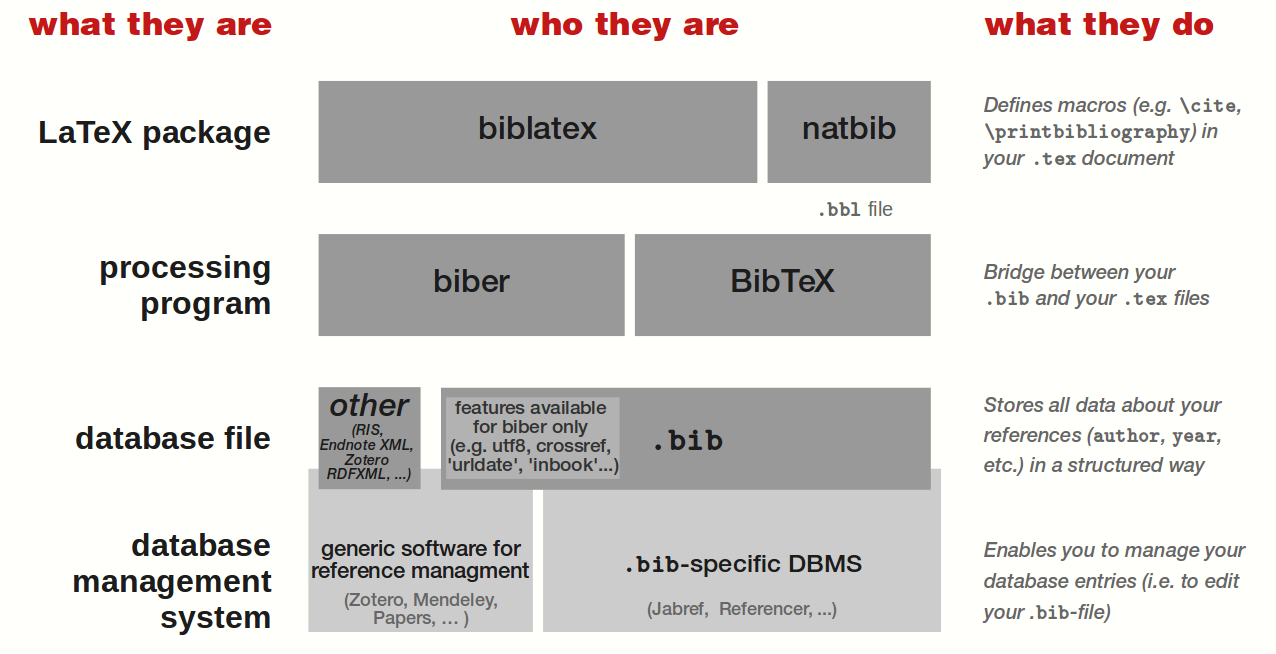
\includegraphics[width=0.8\textwidth]{citations_overview.png}
    \caption{Bibliography Process Overview in \LaTeX}
    \label{fig:bibliography-process}
\end{figure}

At the highest level, there are two main front-end \LaTeX\ packages that users interact with to handle citations, references, and bibliographies. These are \texttt{natbib} and \texttt{biblatex}. \texttt{natbib} is an older package, and although still maintained, may not be further developed. Despite this, it is still widely used, and very reliable in nature.
\texttt{biblatex} is a newer package that is more flexible and can handle more complex bibliography styles, and happens to be actively developed alongside the \texttt{biber} processing program (backend, more on this below). The humanities fields tend to use \texttt{biblatex} as many predefined styles are available (e.g., APA, MLA, Chicago). Science fields tend to go either way depending on the publishing journal's requirements and specific functionalities needed.

The backend or processing programs are the bridge between the \LaTeX\ document and the bibliography file. The two main programs are \texttt{bibtex} and \texttt{biber}. \texttt{bibtex} interfaces with specific \file{.bst} files, which are postfix language files that define the formatting of the bibliography. In the case of many major publication journals (especially in astronomy), the submission of manuscripts require the use of these \file{.bst} files, and as such, users are required to use the \texttt{natbib} \LaTeX\ package. \texttt{biber} on the other hand is a relatively newer processing program that adds further functionality to \texttt{biblatex}.

It is important to note that the \texttt{biblatex} package can make use of either the \texttt{biber} backend or the \texttt{bibtex} backend, while the \texttt{natbib} package is restricted to the \texttt{bibtex} backend. Even more importantly, results with \texttt{biblatex} can differ depending on the backend: if \texttt{bibtex} is used, it only uses it for sorting, and not for formatting content.

The takeaway is the following: if you enjoy a particular style given in a particular journal, download its \file{.bst} file and make use of the \texttt{natbib} package to compile your thesis work.

\section{Choosing a Bibliography Package}
\label{sec:bib-choosing}

The template loads the bibliography package for you, chosen with the \texttt{bibliography} class option. By default (\texttt{bibliography=none}) no bibliography package is loaded at all, so you must choose one before you can cite anything. Whichever you choose, the class adds the bibliography to the table of contents for you, as UVic requires.

\subsection{natbib}

With \texttt{bibliography=natbib}, choose a \file{.bst} style and name your \file{.bib} file at the point where the bibliography should appear. This is how the bibliography of this document is produced, using the \file{aasjournal.bst} style of the AAS journals, which is kept in the \file{extras/} folder:
\begin{lstlisting}[language=TeX]
\documentclass[bibliography=natbib]{uvicphysastro}
...
\bibliographystyle{extras/aasjournal}  % uses extras/aasjournal.bst
\bibliography{references}              % uses references.bib
\end{lstlisting}
A style file kept in \file{extras/} must be named with its folder, as above; a style file placed next to \file{thesis.tex} is named on its own (\cmd{bibliographystyle}\texttt{\{aasjournal\}}).

\texttt{natbib} provides two main citation commands: \cmd{citet} for a citation in the running text, such as \citet{Hubble1929}, and \cmd{citep} for a parenthetical citation, such as \citep{Hubble1929}.

\subsection{Numbered Citations}
\label{sec:bib-numbered}

Physics journals usually cite by number, as in ``[3, 7--9]'', rather than by author and year. With \texttt{natbib}, this needs two package options: \texttt{numbers}, and \texttt{sort\&compress}, which sorts the numbers in each citation and shortens runs such as 7, 8, 9 to 7--9. The class loads \texttt{natbib} itself, so pass the options on the first line of \file{thesis.tex}, before \cmd{documentclass} (Section~\ref{sec:packages}):
\begin{lstlisting}[language=TeX]
\PassOptionsToPackage{numbers,sort&compress}{natbib}
\documentclass[bibliography=natbib]{uvicphysastro}
\end{lstlisting}
Then cite with \cmd{citep} or \cmd{cite}. Combine this with a numbered style such as the APS style (Section~\ref{sec:bib-aps}). Do not also load the \texttt{cite} package, which older documents often use for the same purpose: \texttt{natbib} already sorts and compresses numbered citations, and warns that \texttt{cite} should not be used with it.

\subsection{biblatex}

With \texttt{bibliography=biblatex}, the class loads \texttt{biblatex} with the \texttt{biber} backend, in the style given by the \texttt{bibstyle} class option (\texttt{authoryear} by default). Name your \file{.bib} file in the preamble, and print the bibliography where it should appear:
\begin{lstlisting}[language=TeX]
\documentclass[bibliography=biblatex, bibstyle=authoryear]{uvicphysastro}
\addbibresource{references.bib}
...
\printbibliography
\end{lstlisting}
Citations use \cmd{textcite} (in the text) and \cmd{parencite} (in parentheses).

Use the citation commands of the package you chose: the \texttt{natbib} commands \cmd{citet} and \cmd{citep} are not available with \texttt{biblatex}, and \cmd{textcite} and \cmd{parencite} are not available with \texttt{natbib}. If you switch packages, replace the citation commands in your chapters as well.

\section{Journal Bibliography Styles}
\label{sec:bib-styles}

UVic does not prescribe a citation or bibliography style; follow the style guide of your field, and agree on a style with your supervisor. In astronomy, the easiest choice is usually the style of a journal you publish in, so that your thesis references look like those in your papers. With \texttt{natbib}, a journal style is a single \file{.bst} file chosen with \cmd{bibliographystyle}.

\subsection{Styles Included With the Template}

The \file{extras/} folder contains the styles of two major astronomy journals and of the American Physical Society journals (Table~\ref{tab:bib-styles}). All three are distributed under the \LaTeX\ Project Public License. The AAS and MNRAS styles are included unchanged, and are also part of every full \TeX\ installation (including Overleaf), so \cmd{bibliographystyle}\texttt{\{mnras\}} works even without the copy in \file{extras/}; the copies make sure that you use the versions this template was tested with. The APS style is a corrected copy (Section~\ref{sec:bib-aps}).

\begin{table}[htbp]
    \centering
    \caption{Journal bibliography styles included in \texttt{extras/}.}
    \label{tab:bib-styles}
    \begin{tabularx}{\linewidth}{@{}>{\raggedright\arraybackslash}X l >{\raggedright\arraybackslash}p{0.16\linewidth}@{}}
        \toprule
        Journals & Command & Version \\
        \midrule
        AAS journals (ApJ, ApJL, ApJS, AJ, PSJ) & \cmd{bibliographystyle}\texttt{\{extras/aasjournal\}} & June 2019 (AASTeX 6.3) \\
        MNRAS & \cmd{bibliographystyle}\texttt{\{extras/mnras\}} & v3.2, July 2023 \\
        APS journals (Phys.\ Rev.\ A--E, PRL, \ldots) & \cmd{bibliographystyle}\texttt{\{extras/apsrev4-2-fixed\}} & REVTeX 4.2f, corrected \\
        \bottomrule
    \end{tabularx}
\end{table}

The AAS style is deliberately the 2019 version. AAS distributes a newer \file{aasjournalv7.bst} with AASTeX~7, but it is written for the AASTeX~7 document class: used with any other class, it adds first initials to in-text citations (``E. Hubble (1929)'') and leaves stray spaces and commas in the citations and reference list.

To switch styles, change the \cmd{bibliographystyle} line and compile again; \texttt{latexmk} and Overleaf rerun BibTeX automatically.

\subsection{Physics Journals (APS)}
\label{sec:bib-aps}

The \emph{Physical Review} journals of the American Physical Society use the style \file{apsrev4-2.bst} from REVTeX, which is common in theoretical physics. It numbers the references, so use it with numbered citations (Section~\ref{sec:bib-numbered}):
\begin{lstlisting}[language=TeX]
\PassOptionsToPackage{numbers,sort&compress}{natbib}
\documentclass[bibliography=natbib]{uvicphysastro}
...
\bibliographystyle{extras/apsrev4-2-fixed}
\bibliography{references}
\end{lstlisting}
The first line passes the \texttt{numbers} and \texttt{sort\&compress} options to \texttt{natbib}: it must come before \cmd{documentclass}, because the class loads \texttt{natbib} itself.

The file is a corrected copy of \file{apsrev4-2.bst}, hence the name \file{-fixed} (the \LaTeX\ Project Public License requires a modified file to be renamed). Outside the REVTeX document class, the original style leaves a stray space before the final full stop of every reference with an arXiv number, as in ``arXiv:1807.06209 [astro-ph.CO]~.''; the copy removes that space and changes nothing else. The change is described at the top of the file.

\subsection{Other Styles}

\begin{description}
    \item[\texttt{natbib}'s own styles.] \texttt{plainnat}, \texttt{abbrvnat} and \texttt{unsrtnat} come with every \TeX\ installation and give general-purpose author--year references. Avoid \LaTeX's basic styles \texttt{plain}, \texttt{abbrv} and \texttt{unsrt} with \texttt{natbib}: they give numbered references without author names, so \cmd{citet} prints ``(author?)~[4]'' instead of the author.
    \item[Other journals.] Most journals provide a \file{.bst} file with their \LaTeX\ instructions for authors. For example, the style of \emph{Astronomy \& Astrophysics}, \file{aa.bst}, is part of the A\&A macro package available from the A\&A website (\url{https://www.aanda.org}). It is not included in this template because its licence terms do not clearly permit redistribution. Download the style, place the \file{.bst} file in \file{extras/} (or next to \file{thesis.tex}), and select it as above.
\end{description}

\section{Journal Abbreviations in \texttt{.bib} Files}
\label{sec:bib-journal-macros}

Most astronomers collect their references from the NASA Astrophysics Data System (ADS, \url{https://ui.adsabs.harvard.edu}), which exports BibTeX entries ready to paste into \file{references.bib}. For many journals, ADS writes the journal name as a \LaTeX\ macro rather than as text:
\begin{lstlisting}[language=TeX]
@ARTICLE{Planck2020,
  author = {{Planck Collaboration} and {Aghanim}, N. and {Akrami}, Y. and others},
  title = "{Planck 2018 results. VI. Cosmological parameters}",
  journal = {\aap},
  year = 2020,
  volume = {641},
  eid = {A6},
  doi = {10.1051/0004-6361/201833910},
}
\end{lstlisting}
The macro \cmd{aap} stands for \emph{Astronomy \& Astrophysics}. Journal document classes such as AASTeX and the A\&A and MNRAS classes define these macros, but standard \LaTeX\ does not: in an ordinary document, a reference to a paper in A\&A, ApJ or MNRAS stops compilation with an ``Undefined control sequence'' error.

This class defines every journal macro on ADS's list (\url{https://ui.adsabs.harvard.edu/help/actions/journal-macros}), so references exported from ADS work without any changes. Each macro prints the journal's standard abbreviation, as in the AAS and A\&A journals; Table~\ref{tab:journal-macros} shows the most common ones, and the full list is in \file{uvicphysastro.cls}. Journals that are not on ADS's list (such as \emph{Nature Astronomy} or \emph{JATIS}) are exported with their name written out in full, so they need no macro. ADS also writes the symbols $\lesssim$ and $\gtrsim$ in paper titles as the macros \cmd{lessequivlnt} and \cmd{greaterequivlnt}, which the class defines as well.

\begin{table}[htbp]
    \centering
    \caption[Common journal macros used in ADS BibTeX entries]{Common journal macros used in ADS BibTeX entries, and what they print.}
    \label{tab:journal-macros}
    \begin{tabularx}{\linewidth}{@{}l >{\raggedright\arraybackslash}X l@{}}
        \toprule
        Macro & Journal & Prints \\
        \midrule
        \cmd{apj}, \cmd{apjl}, \cmd{apjs} & Astrophysical Journal (Letters, Supplement) & \apj, \apjl, \apjs \\
        \cmd{aj} & Astronomical Journal & \aj \\
        \cmd{mnras} & Monthly Notices of the RAS & \mnras \\
        \cmd{aap} & Astronomy \& Astrophysics & \aap \\
        \cmd{araa} & Annual Review of Astronomy and Astrophysics & \araa \\
        \cmd{pasp} & Publications of the ASP & \pasp \\
        \cmd{pasa} & Publications of the ASA & \pasa \\
        \cmd{psj} & Planetary Science Journal & \psj \\
        \cmd{jcap} & J.\ Cosmology and Astroparticle Physics & \jcap \\
        \cmd{nat} & Nature & \nat \\
        \cmd{prd} & Physical Review D & \prd \\
        \cmd{procspie} & Proceedings of the SPIE & \procspie \\
        \bottomrule
    \end{tabularx}
\end{table}

If you would rather show full journal names, redefine the macro in the preamble of \file{thesis.tex}, for example \cmd{renewcommand}\texttt{\{\textbackslash apj\}\{Astrophysical Journal\}}, or replace the macro in your \file{.bib} file with the name written out.

\chapter{Tables}
\label{ch:tables}

Similarly with other topics in \LaTeX, there are a multitude of different ways to achieve the same output. As with most basic implementations, Overleaf has fantastic resources. The following link is a great place to start for basic and slightly more advanced table implementations: \url{https://www.overleaf.com/learn/latex/Tables}.

\section{Comprehensive Tables}
\label{sec:tables-comprehensive}

This section will cover what I believe is a fantastic way to implement basic and complex tables, using standard \LaTeX\ packages. If you are used to the \texttt{deluxetable} environment from AASTeX, note that this template does not support it; the examples below show how to build the same kinds of tables (table notes, tables that continue over several pages, landscape tables) with standard packages.

While the generic \texttt{tabular} environment is a great place to start, it does not account for the complex table implementations that I needed (tables with merged cells, tables that spilled over pages, landscape tables, etc.).

The following is a list of the packages that allowed me the most flexibility in creating tables that I needed for my thesis. These are in order of the most basic to the most complex:

\subsection{Basis Packages}
\label{sec:tables-basis-packages}

These are what I describe as basis packages, which add in the ability to create tables that are more complex than the basic \texttt{tabular} environment, but are not as complex as the packages that will be discussed later in this section, which essentially have the abilities to \emph{merge} these environments together under one umbrella environment.


\begin{itemize}
    \item \texttt{longtable} - Allows the ability for tables to continue onto the next page. This is great for tables that are too long to fit on a single page.
    \item \texttt{tabularx} - Allows the column designator \texttt{x} to be used, which will automatically adjust the column width in order for the table to fill the declared width of the environment.
    \item \texttt{threeparttable} - Provides a scheme for tables that have a structured note section after the caption.
    \item \texttt{booktabs} - Provides some additional commands to enhance the quality of tables.
    \item \texttt{caption} - Provides the ability to customize the caption of the table. Specifically useful for tables that are too long to fit on a single page (continued captions).
    \item \texttt{multirow} - Provides the ability to merge cells in the row direction.
    \item \texttt{pdflscape} - Provides the ability to create landscape tables.
\end{itemize}

\subsection{Extension Packages}
\label{sec:tables-extension-packages}

As mentioned above, these packages are extensions of the basic packages, and allow for more complex table implementations. These are what made all the different packages work together in a seamless way.

\begin{itemize}
    \item \texttt{threeparttablex} - This package extends the \texttt{threeparttable} package to work with tables created using the \texttt{longtable} package.
    \item \texttt{xltabular} - This package extends the \texttt{longtable} and \texttt{tabularx} packages to work together. Introduces the \texttt{xltabular} environment.
\end{itemize}

\section{Example Tables}
\label{sec:tables-example}

Here is a regular \texttt{tabular} environment, modified by the \texttt{booktabs} package. This is a great way to start creating tables, as it is simple and easy to understand. The \texttt{booktabs} package provides some additional commands to enhance the quality of tables such as the \texttt{toprule}, \texttt{midrule}, and \texttt{bottomrule} commands.

The following is the templated code for the table:

\lstinputlisting[language=TeX]{content/examples/table_simpletable.tex}

The compiled from the above templated code is the following:

\begin{table}[htbp]
    \centering
    \begin{tabular}{cccccccc}
        \toprule
        {$m$} & {$M_\odot$} & {$R_\odot$} & {$L_\odot$} & {$A_\nu$} & {$A_m$} & {$\varphi(m)$} & {$\varphi(a)$} \\ \midrule
        1  & 16.128 & +8.872 & 16.128 & 1.402 & 1.373 & -146.6 & -137.6 \\
        2  & 3.442  & -2.509 & 3.442  & 0.299 & 0.343 & 133.2  & 152.4  \\ \midrule
        3  & 1.826  & -0.363 & 1.826  & 0.159 & 0.119 & 168.5  & -161.1 \\
        4  & 0.993  & -0.429 & 0.993  & 0.086 & 0.08  & 25.6   & 90     \\ \bottomrule
    \end{tabular}
\end{table}

Extending this to use a \texttt{threeparttable} environment, including a caption and notes, would be the following:

\lstinputlisting[language=TeX]{content/examples/table_threeparttable.tex}

The compiled from the above templated code is the following:

\begin{table}[htbp]
    \centering
    \begin{threeparttable}
        \caption{Example Table with ThreePartTable and Caption
        \label{tab:example-threeparttable}}
        \begin{tabular}{cccccccc}
            \toprule
            {$m$} & {$M_\odot$} & {$R_\odot$} & {$L_\odot$} & {$A_\nu$} & {$A_m$} & {$\varphi(m)$} & {$\varphi(a)$} \\ \midrule
            1  & 16.128 & +8.872 & 16.128 & 1.402 & 1.373 & -146.6 & -137.6 \\
            2  & 3.442  & -2.509 & 3.442  & 0.299 & 0.343 & 133.2  & 152.4  \\ \midrule
            3  & 1.826  & -0.363 & 1.826  & 0.159 & 0.119 & 168.5  & -161.1 \\
            4  & 0.993  & -0.429 & 0.993  & 0.086 & 0.08  & 25.6   & 90     \\ \bottomrule
        \end{tabular}
        %
        \begin{tablenotes}[flushleft]
            \footnotesize
            \item \textbf{First Note:} This is a note.
            \item \textit{Second Notes:} This is also a note.
        \end{tablenotes}
    \end{threeparttable}
\end{table}

Expanding now to use the \texttt{tabularx} environment for automatic re-sizing of the columns. For reference, in this example, all columns but the first use the \texttt{X} designation. The following code would be used:

\lstinputlisting[language=TeX]{content/examples/table_tabularx.tex}

The compiled from the above templated code is the following:

\begin{table}[htbp]
    \centering
    \begin{threeparttable}
        \caption{Example Table with ThreePartTable and Caption
        \label{tab:example-tabularx}}
        \begin{tabularx}{\textwidth}{cXXXXXXX}
            \toprule
            {$m$} & {$M_\odot$} & {$R_\odot$} & {$L_\odot$} & {$A_\nu$} & {$A_m$} & {$\varphi(m)$} & {$\varphi(a)$} \\ \midrule
            1  & 16.128 & +8.872 & 16.128 & 1.402 & 1.373 & -146.6 & -137.6 \\
            2  & 3.442  & -2.509 & 3.442  & 0.299 & 0.343 & 133.2  & 152.4  \\ \midrule
            3  & 1.826  & -0.363 & 1.826  & 0.159 & 0.119 & 168.5  & -161.1 \\
            4  & 0.993  & -0.429 & 0.993  & 0.086 & 0.08  & 25.6   & 90     \\ \bottomrule
        \end{tabularx}
        %
        \begin{tablenotes}[flushleft]
            \footnotesize
            \item First Note: This is a note.
            \item Second Notes: This is also a note.
        \end{tablenotes}
    \end{threeparttable}
\end{table}

The last example will be a combination of all the above packages, including the \texttt{longtable} package to allow the table to continue onto the next page, the \texttt{multirow} package to merge cells in the row direction, and the \texttt{pdflscape} package to create a landscape table. The following code will be used (data and header information have been selectively trimmed for readability):

\lstinputlisting[language=TeX]{content/examples/table_complex_trimmed.txt}

\begin{landscape}
    \begin{ThreePartTable}
        \begin{TableNotes}[flushleft, para]
            \footnotesize
            $^{\text{a}}$ Properties of the Gaussian fit to the ALMA emission: peak flux, integrated flux, major and minor axes of the FWHM, and position angle of the FWHM. \\
            $^{\text{b}}$ Properties of the deconvolved Gaussian fit: major and minor axes of the FWHM, and position angle of the FWHM. Unresolved sources are indicated by values of -1.
        \end{TableNotes}
        \centering
        \scriptsize
        \setlength{\tabcolsep}{4pt}  % tighter columns so all 16 fit across the page
        \begin{xltabular}{\linewidth}{Xccccccccccccccc}
            \caption{Example Table with ThreePartTable, LongTable, Caption, Notes, Landscape\label{tab:observed-properties}}\\
            \toprule
            Scr &  R.A.  &  Decl. & Pk$^{\text{a}}$ & Pk$_{\text{err}}$$^{\text{a}}$ & Tot$^{\text{a}}$ & Tot$_{\text{err}}$$^{\text{a}}$ & FWHM$_{\text{a}}$$^{\text{a}}$ & FWHM$_{\text{b}}$$^{\text{a}}$ &  P.A.$^{\text{a}}$ & \multicolumn{2}{c}{FWHM$_{\text{a,d}}$$^{\text{b}}$ (arcsec)} & \multicolumn{2}{c}{FWHM$_{\text{b,d}}$$^{\text{b}}$ (arcsec)} & \multicolumn{2}{c}{P.A.$_{\text{d}}$$^{\text{b}}$ (deg)}\\
            & (J2000) & (J2000) & \multicolumn{2}{c}{($\text{mJy}~\text{beam}^{-1}$)} & \multicolumn{2}{c}{($\text{mJy}$)} & \multicolumn{2}{c}{(arcsec)} & (deg) & fit & err & fit & err & fit & err \\
            \midrule
            \endfirsthead
            
            \caption[]{(continued from previous page)} \\
            \toprule
            Scr &  R.A.  &  Decl. & Pk$^{\text{a}}$ & Pk$_{\text{err}}$$^{\text{a}}$ & Tot$^{\text{a}}$ & Tot$_{\text{err}}$$^{\text{a}}$ & FWHM$_{\text{a}}$$^{\text{a}}$ & FWHM$_{\text{b}}$$^{\text{a}}$ &  P.A.$^{\text{a}}$ & \multicolumn{2}{c}{FWHM$_{\text{a,d}}$$^{\text{b}}$ (arcsec)} & \multicolumn{2}{c}{FWHM$_{\text{b,d}}$$^{\text{b}}$ (arcsec)} & \multicolumn{2}{c}{P.A.$_{\text{d}}$$^{\text{b}}$ (deg)}\\
            & (J2000) & (J2000) & \multicolumn{2}{c}{($\text{mJy}~\text{beam}^{-1}$)} & \multicolumn{2}{c}{($\text{mJy}$)} & \multicolumn{2}{c}{(arcsec)} & (deg) & fit & err & fit & err & fit & err \\
            \midrule
            \endhead
            
            \bottomrule
            \multicolumn{16}{r}{\footnotesize to be continued on the next page}
            \endfoot
            
            \bottomrule
            \insertTableNotes
            \endlastfoot
            
            1  &  05h46m06.01s &  -00d09m32.70s &  0.36 &    0.08 &  4.60 &     1.03 & 5.471 & 4.622 &  58.8 &  5.26 &    1.22 &  4.43 &    1.07 &   58 &      53 \\
            2  &  05h46m07.26s &  -00d13m30.27s &  9.48 &    0.16 & 12.22 &     0.33 & 1.849 & 1.511 &  71.2 &  0.84 &    0.09 &  0.74 &    0.08 &   65 &      66 \\
            3  &  05h46m07.33s &  -00d13m43.49s & 31.37 &    0.16 & 36.88 &     0.31 & 1.779 & 1.433 &  70.1 &  0.68 &    0.03 &  0.56 &    0.03 &   57 &      12 \\
            4  &  05h46m07.51s &  -00d13m54.79s &  0.45 &    0.16 &  1.36 &     0.63 & 2.978 & 2.177 & 162.1 &  2.67 &    1.19 &  1.42 &    1.04 &  162 &      42 \\
            5  &  05h46m07.53s &  -00d11m49.22s &  0.97 &    0.14 &  5.25 &     0.90 & 4.345 & 2.694 & 152.4 &  4.14 &    0.74 &  2.14 &    0.49 &  153 &      11 \\
            6  &  05h46m07.73s &  -00d12m21.27s & 14.37 &    0.17 & 21.73 &     0.38 & 1.977 & 1.658 &  82.8 &  1.15 &    0.06 &  0.94 &    0.06 &  110 &      12 \\
            7  &  05h46m07.84s &  -00d09m59.61s &  6.45 &    0.11 &  7.59 &     0.21 & 1.726 & 1.361 &  65.2 &  0.81 &    0.07 &  0.36 &    0.10 &   62 &       8 \\
            8  &  05h46m07.86s &  -00d10m01.33s &  2.74 &    0.11 &  3.44 &     0.23 & 1.754 & 1.427 &  63.0 &  0.88 &    0.17 &  0.56 &    0.23 &   57 &      48 \\
            9  &  05h46m08.42s &  -00d10m01.03s &  0.86 &    0.09 &  5.53 &     0.69 & 4.752 & 2.702 &  38.9 &  4.52 &    0.60 &  2.33 &    0.34 &   38 &       8 \\
            10 &  05h46m08.49s &  -00d10m03.10s &  8.13 &    0.10 &  7.55 &     0.17 & 1.444 & 1.284 &  83.2 & -1.00 &   -1.00 & -1.00 &   -1.00 &   -1 &      -1 \\
            11 &  05h46m08.92s &  -00d09m56.11s &  2.07 &    0.11 &  2.28 &     0.20 & 1.576 & 1.392 &  73.8 &  0.51 &    0.31 &  0.36 &    0.21 &  129 &      73 \\
            12 &  05h46m10.04s &  -00d12m16.83s & 39.04 &    0.15 & 40.36 &     0.28 & 1.657 & 1.352 &  72.0 &  0.31 &    0.03 &  0.19 &    0.09 &  165 &      24 \\
            13 &  05h46m13.13s &  -00d06m04.94s &  9.41 &    0.14 & 11.18 &     0.27 & 1.655 & 1.379 &  67.3 &  0.71 &    0.07 &  0.50 &    0.08 &   60 &      19 \\
            14 &  05h46m14.20s &  -00d05m26.71s &  0.51 &    0.13 &  0.54 &     0.24 & 1.704 & 1.177 &  80.5 & -1.00 &   -1.00 & -1.00 &   -1.00 &   -1 &      -1 \\
            15 &  05h46m27.91s &  -00d00m52.11s & 65.62 &    0.14 & 73.72 &     0.27 & 1.662 & 1.409 &  74.0 &  0.52 &    0.02 &  0.49 &    0.02 &   43 &      26 \\
            16 &  05h46m28.34s &  +00d19m49.18s &  1.47 &    0.14 &  1.79 &     0.28 & 1.816 & 1.387 &  78.5 &  0.93 &    0.36 &  0.42 &    0.27 &   77 &      82 \\
            17 &  05h46m28.61s &  +00d20m58.08s &  0.50 &    0.13 &  0.49 &     0.23 & 1.675 & 1.212 & 127.5 &  0.00 &    1.59 &  0.00 &    0.60 &   -1 &      -1 \\
            18 &  05h46m30.91s &  -00d02m35.07s &  7.55 &    0.15 & 17.54 &     0.47 & 2.456 & 1.972 &  63.7 &  1.89 &    0.07 &  1.45 &    0.06 &   58 &       7 \\
            19 &  05h46m31.09s &  -00d02m32.95s & 16.15 &    0.15 & 25.05 &     0.35 & 1.862 & 1.736 & 151.5 &  1.31 &    0.03 &  0.73 &    0.05 &  160 &       5 \\
            20 &  05h46m43.12s &  +00d00m52.47s &  1.70 &    0.13 &  2.40 &     0.28 & 1.759 & 1.619 &   2.1 &  1.15 &    0.33 &  0.56 &    0.42 &  169 &      36 \\
            21 &  05h46m46.52s &  +00d00m16.09s &  1.00 &    0.12 &  1.04 &     0.22 & 1.532 & 1.370 &  63.8 &  0.00 &    1.05 &  0.00 &    0.50 &   -1 &      -1 \\
            22 &  05h46m47.03s &  +00d00m27.20s &  1.96 &    0.13 &  3.55 &     0.34 & 2.212 & 1.652 & 109.8 &  1.69 &    0.25 &  0.83 &    0.30 &  118 &      13 \\
            23 &  05h46m47.43s &  +00d00m23.24s &  1.10 &    0.09 & 12.48 &     1.10 & 5.314 & 4.321 &  37.9 &  5.11 &    0.47 &  4.09 &    0.39 &   36 &      22 \\
            24 &  05h46m47.51s &  +00d00m29.50s &  0.85 &    0.10 &  7.75 &     1.04 & 5.548 & 3.319 &   9.5 &  5.38 &    0.75 &  2.97 &    0.45 &    9 &       9 \\
            25 &  05h46m47.69s &  +00d00m25.02s &  5.38 &    0.13 &  7.22 &     0.27 & 1.810 & 1.496 &  53.6 &  1.01 &    0.11 &  0.64 &    0.13 &   37 &      15 \\
            26 &  05h46m47.97s &  +00d01m41.80s &  1.10 &    0.13 &  2.55 &     0.42 & 2.665 & 1.684 &  38.5 &  2.24 &    0.48 &  0.99 &    0.43 &   34 &      15 \\
            27 &  05h46m57.30s &  +00d23m57.94s &  3.39 &    0.16 &  4.25 &     0.33 & 1.666 & 1.417 &  72.1 &  0.83 &    0.21 &  0.55 &    0.34 &   61 &      72 \\
            28 &  05h47m00.92s &  +00d26m21.98s &  2.65 &    0.16 &  9.34 &     0.71 & 2.782 & 2.363 & 161.4 &  2.46 &    0.21 &  1.87 &    0.19 &  163 &      15 \\
            29 &  05h47m01.31s &  +00d26m23.09s &  4.91 &    0.17 &  6.96 &     0.37 & 1.784 & 1.484 &  92.6 &  1.05 &    0.12 &  0.72 &    0.13 &   99 &      21 \\
            30 &  05h47m10.61s &  +00d21m13.78s & 12.17 &    0.16 & 16.31 &     0.35 & 1.755 & 1.491 &  83.6 &  0.93 &    0.06 &  0.70 &    0.06 &   94 &      12 \\
            31 &  05h47m15.95s &  +00d21m22.89s &  2.02 &    0.13 &  2.70 &     0.28 & 1.805 & 1.553 &  89.0 &  0.92 &    0.29 &  0.75 &    0.51 &  111 &      77 \\
            32 &  05h47m24.84s &  +00d20m58.98s & 16.42 &    0.15 & 51.09 &     0.60 & 2.773 & 2.400 & 133.8 &  2.39 &    0.04 &  1.84 &    0.04 &  144 &       3 \\
            33 &  05h47m32.45s &  +00d20m21.60s &  5.56 &    0.15 &  7.19 &     0.30 & 1.742 & 1.502 &  98.7 &  0.91 &    0.14 &  0.60 &    0.20 &  129 &      21 \\
            34 &  05h47m36.56s &  +00d20m05.89s &  8.36 &    0.15 & 10.28 &     0.29 & 1.651 & 1.508 &  79.1 &  0.75 &    0.07 &  0.58 &    0.12 &  173 &      35 \\
            34 &  05h47m36.56s &  +00d20m05.89s &  8.36 &    0.15 & 10.28 &     0.29 & 1.651 & 1.508 &  79.1 &  0.75 &    0.07 &  0.58 &    0.12 &  173 &      35 \\
            34 &  05h47m36.56s &  +00d20m05.89s &  8.36 &    0.15 & 10.28 &     0.29 & 1.651 & 1.508 &  79.1 &  0.75 &    0.07 &  0.58 &    0.12 &  173 &      35 \\
            34 &  05h47m36.56s &  +00d20m05.89s &  8.36 &    0.15 & 10.28 &     0.29 & 1.651 & 1.508 &  79.1 &  0.75 &    0.07 &  0.58 &    0.12 &  173 &      35 \\
            34 &  05h47m36.56s &  +00d20m05.89s &  8.36 &    0.15 & 10.28 &     0.29 & 1.651 & 1.508 &  79.1 &  0.75 &    0.07 &  0.58 &    0.12 &  173 &      35 \\
            34 &  05h47m36.56s &  +00d20m05.89s &  8.36 &    0.15 & 10.28 &     0.29 & 1.651 & 1.508 &  79.1 &  0.75 &    0.07 &  0.58 &    0.12 &  173 &      35 \\
        \end{xltabular}
    \end{ThreePartTable}
\end{landscape}

\chapter{Figures and Astronomical Notation}
\label{ch:astronomy}

\section{Figures}
\label{sec:figures}

Place your images in \file{content/figures/}. Because \file{thesis.tex} sets \cmd{graphicspath} to that folder, \cmd{includegraphics} only needs the file name. Figure~\ref{fig:bibliography-process} in Chapter~\ref{ch:bibliographies} was included with:
\begin{lstlisting}[language=TeX]
\begin{figure}[htbp]
    \centering
    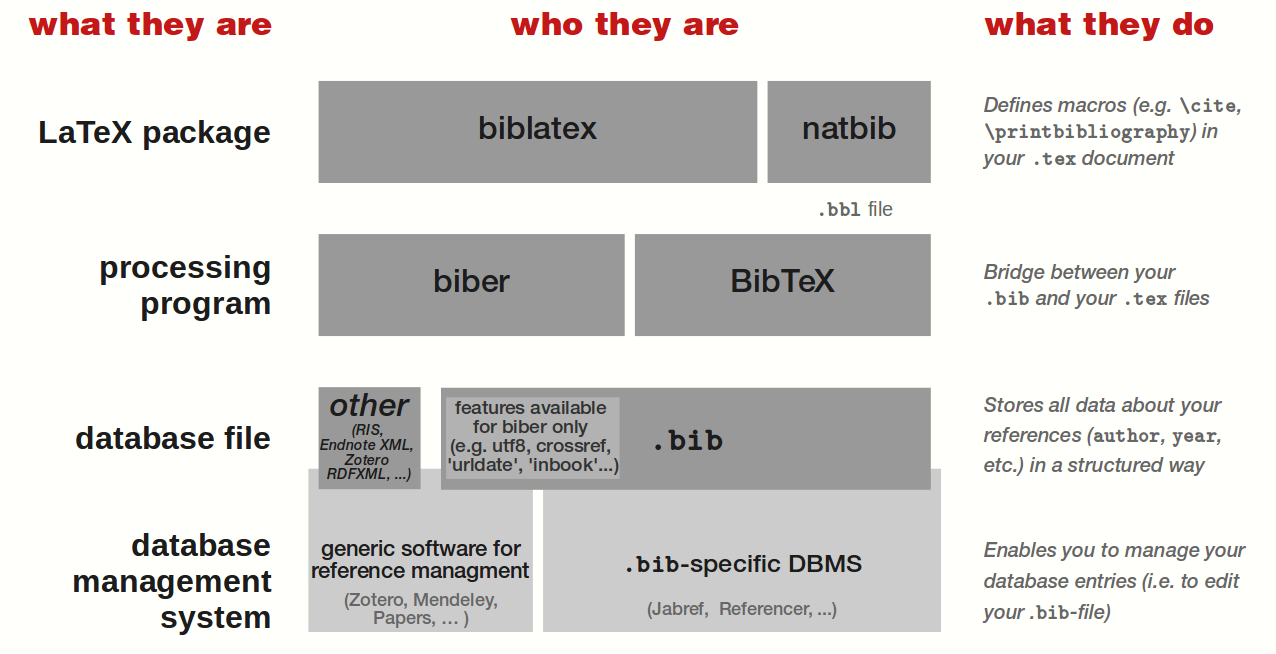
\includegraphics[width=0.8\textwidth]{citations_overview.png}
    \caption{Bibliography Process Overview in \LaTeX}
    \label{fig:bibliography-process}
\end{figure}
\end{lstlisting}
Always give a figure a \cmd{caption} (this is what appears in the List of Figures) and a \cmd{label}, and refer to it in the text with \cmd{ref}. Figures with several panels can use the \texttt{subfigure} environment from the \texttt{subcaption} package, which the class loads. Vector formats (PDF) stay sharp at any zoom level; use PNG or JPEG only for photographs and images.

\section{Astronomical Notation}
\label{sec:notation}

The class provides the notation macros of the AASTeX journal class, so that text using them can be copied from a paper written with AASTeX. They work in normal text; Table~\ref{tab:notation} lists them.

\begin{table}[htbp]
    \centering
    \caption[Astronomical notation macros provided by the class]{Astronomical notation macros provided by the class.}
    \label{tab:notation}
    \begin{tabularx}{\linewidth}{@{}l l >{\raggedright\arraybackslash}X@{}}
        \toprule
        Command & Output & Meaning \\
        \midrule
        \cmd{arcdeg}, \cmd{degr} & 5\arcdeg & degrees \\
        \cmd{arcmin} & 5\arcmin & arcminutes \\
        \cmd{arcsec} & 5\arcsec & arcseconds \\
        \cmd{fd}, \cmd{fh}, \cmd{fm}, \cmd{fs} & 2\fd5, 12\fh5, 30\fm5, 45\fs5 & fractional day, hour, minute, second \\
        \cmd{fdg}, \cmd{farcm}, \cmd{farcs} & 3\fdg2, 4\farcm5, 0\farcs75 & fractional degree, arcminute, arcsecond \\
        \cmd{fp} & 1\fp5 & fractional parallax \\
        \cmd{micron} & 2.2~\micron & micrometres \\
        \cmd{ion}\texttt{\{Fe\}\{2\}} & \ion{Fe}{2} & ionization state \\
        \cmd{la}, \cmd{ga} & $z \la 2$, $z \ga 2$ & less / greater than about \\
        \cmd{ubvr}, \cmd{ub}, \cmd{bv}, \cmd{vr}, \cmd{ur} & \ubvr, \ub, \bv, \vr, \ur & photometric bands and colours \\
        \cmd{case}\texttt{\{1\}\{3\}}, \cmd{onehalf} & \case{1}{3}, \onehalf & fractions in running text \\
        \bottomrule
    \end{tabularx}
\end{table}

Note that \cmd{la} and \cmd{ga} must be used in math mode, as in \verb|$z \la 2$|.

For the fractional units, put the macro where the decimal point goes: \verb|12\fh5| gives 12\fh5.

\section{Aligning Numbers in Tables}
\label{sec:phantoms}

The class also provides the AASTeX ``phantom'' commands, which insert invisible space the width of a character so that columns of numbers line up:
\begin{center}
    \begin{tabular}{@{}l l@{}}
        \toprule
        Command & Inserts the width of \\
        \midrule
        \cmd{phn} & a digit \\
        \cmd{phd} & a decimal point \\
        \cmd{phs} & a minus sign \\
        \cmd{phm}\texttt{\{text\}} & any text \\
        \bottomrule
    \end{tabular}
\end{center}

\section{Symbols}
\label{sec:symbols}

Solar units are written in math mode with \verb|\odot|, for example \verb|$M_\odot$| gives $M_\odot$. The \texttt{wasysym} package, loaded by the class, provides further astronomical symbols for use in text, such as \cmd{sun} (\sun), \cmd{mercury} (\mercury), \cmd{venus} (\venus), \cmd{earth} (\earth), \cmd{mars} (\mars), \cmd{jupiter} (\jupiter), and \cmd{saturn} (\saturn). The full list is in the \texttt{wasysym} documentation.


\bibliographystyle{extras/aasjournal}
\bibliography{references}

% Appendices (optional): uncomment, and add one file per appendix
% \appendix
% \include{content/appendixA}

\end{document}
